\documentclass[tikz,border=5pt]{standalone}
\usepackage[T1]{fontenc}
\usepackage{lmodern,amsmath,amssymb}
\usetikzlibrary{arrows.meta,calc,positioning,fit,backgrounds,shapes.geometric,matrix,decorations.pathreplacing,patterns}
\definecolor{ink}{gray}{0.08}
\definecolor{wash}{gray}{0.965}
\definecolor{soft}{gray}{0.45}
\tikzset{box/.style={draw=ink,line width=.65pt,fill=white,align=center,inner sep=4pt,outer sep=0pt,font=\small},flow/.style={draw=ink,line width=.65pt,-{Latex[length=1.8mm,width=1.3mm]},rounded corners=2pt},annotation/.style={font=\scriptsize,text=soft,align=center},groupbox/.style={draw=soft,dashed,line width=.45pt,fill=wash}}
\begin{document}
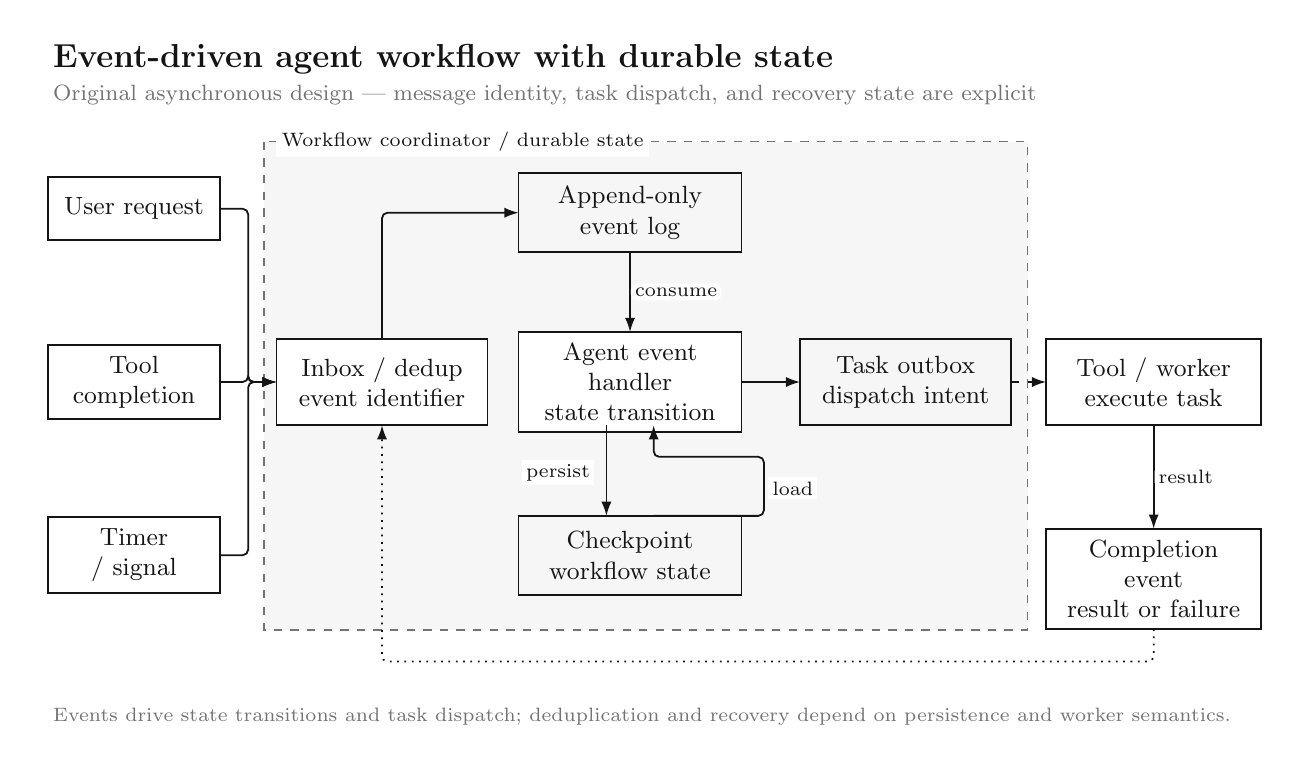
\begin{tikzpicture}[x=1cm,y=-1cm,font=\rmfamily,text=ink]

\path[use as bounding box] (0,0) rectangle (16,9);
\node[anchor=west,font=\large\bfseries] at (.2,.4) {Event-driven agent workflow with durable state};
\node[anchor=west,font=\footnotesize,text=soft] at (.2,.85) {Original asynchronous design | message identity, task dispatch, and recovery state are explicit};
\begin{pgfonlayer}{background}
\draw[groupbox] (3.0,1.45) rectangle (12.7,7.65);
\node[anchor=west,font=\scriptsize,fill=white,inner sep=2pt] at (3.15,1.45) {Workflow coordinator / durable state};
\end{pgfonlayer}
\node[box,minimum width=2.15cm,minimum height=0.8cm,text width=1.9cm] (user) at (1.35,2.3) {User request};
\node[box,minimum width=2.15cm,minimum height=0.8cm,text width=1.9cm] (tool) at (1.35,4.5) {Tool completion};
\node[box,minimum width=2.15cm,minimum height=0.8cm,text width=1.9cm] (timer) at (1.35,6.7) {Timer / signal};
\node[box,minimum width=2.65cm,minimum height=1.1cm,text width=2.4cm] (inbox) at (4.5,4.5) {Inbox / dedup\\event identifier};
\node[box,fill=wash,minimum width=2.8cm,minimum height=1.0cm,text width=2.55cm] (log) at (7.65,2.35) {Append-only\\event log};
\node[box,minimum width=2.8cm,minimum height=1.1cm,text width=2.55cm] (handler) at (7.65,4.5) {Agent event handler\\state transition};
\node[box,fill=wash,minimum width=2.8cm,minimum height=1.0cm,text width=2.55cm] (checkpoint) at (7.65,6.7) {Checkpoint\\workflow state};
\node[box,fill=wash,minimum width=2.65cm,minimum height=1.1cm,text width=2.4cm] (outbox) at (11.15,4.5) {Task outbox\\dispatch intent};
\node[box,minimum width=2.7cm,minimum height=1.1cm,text width=2.45cm] (worker) at (14.3,4.5) {Tool / worker\\execute task};
\node[box,minimum width=2.7cm,minimum height=1.0cm,text width=2.45cm] (completion) at (14.3,7.0) {Completion event\\result or failure};
\begin{pgfonlayer}{background}
\draw[flow] (user.east) -- (2.8,2.3) -- (2.8,4.5) -- (inbox.west);
\draw[flow] (tool.east) -- (2.8,4.5) -- (2.8,4.5) -- (inbox.west);
\draw[flow] (timer.east) -- (2.8,6.7) -- (2.8,4.5) -- (inbox.west);
\draw[flow] (inbox.north) -- (4.5,2.35) -- (log.west);
\draw[flow] (log.south) -- (handler.north) node[midway,right,fill=white,inner sep=1.5pt,font=\scriptsize] {consume};
\draw[flow] (handler.east) -- (outbox.west);
\draw[flow,dashed] (outbox.east) -- (worker.west);
\draw[flow] (worker.south) -- (completion.north) node[midway,right,fill=white,inner sep=1.5pt,font=\scriptsize] {result};
\draw[flow,dotted] (completion.south) -- (14.3,8.05) -- (4.5,8.05) -- (inbox.south);
\end{pgfonlayer}
\draw[flow] (7.35,5.05) -- (7.35,6.2);
\node[font=\scriptsize,fill=white,inner sep=1.5pt,anchor=east] at (7.2,5.65) {persist};
\draw[flow] (7.95,6.2) -- (9.35,6.2) -- (9.35,5.45) -- (7.95,5.45) -- (7.95,5.05);
\node[font=\scriptsize,fill=white,inner sep=1.5pt,anchor=west] at (9.4,5.85) {load};
\node[anchor=west,align=left,font=\scriptsize,text=soft,text width=15.6cm] at (.2,8.75) {Events drive state transitions and task dispatch; deduplication and recovery depend on persistence and worker semantics.};
\end{tikzpicture}
\end{document}
